\section{Modelo de implantação}

No modelo de implantação, dependemos das necessidades das aplicações que serão
implementadas. A restrição ou abertura de acesso depende do processo de negócios,
do tipo de informação e do nível de visão desejado. Percebemos que certas
organizações não desejam que todos os usuários possam acessar e utilizar
determinados recursos no seu ambiente de computação em nuvem. Abaixo seguem
diferentes tipos de implantação~\cite{ibm-what-is-cloud-computing}:

\subsection{Nuvem privada}

Uma nuvem privada é de propriedade e operada por uma única empresa que controla a 
maneira como recursos virtualizados e serviços automatizados são customizados e 
usados por várias linhas de negócios e grupos 
constituintes~\cite{ibm-what-is-cloud-computing}. Nuvens privadas existem para tirar 
proveito de muitas eficiências da nuvem, enquanto fornecem mais controle de recursos 
e direção sem ocupação variada ~\cite{ibm-what-is-cloud-computing}.

\begin{figure}[ht]
    \centering
    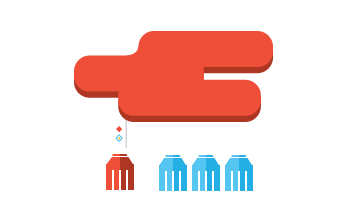
\includegraphics[width=0.4\textwidth]{img/private.png}
    \caption{Nuvem privada~\cite{ibm-what-is-cloud-computing}}
    \label{img:privatecloud}
\end{figure}

Diferentemente de um data center privado virtual, a infraestrutura utilizada
pertence ao usuário. Portanto, ele possui total controle sobre como as aplicações
são implementadas na nuvem. Uma nuvem privada é, em geral, construída sobre um data
center privado ~\cite{technet-cloud-computing}.

Características chave de nuvens privadas incluem~\cite{ibm-what-is-cloud-computing}:

\begin{itemise}
    \item Uma interface de autoatendimento que controla serviços comuns, permitindo
        que a equipe de TI forneça, aloque e entregue rapidamente recursos de TI
        sob demanda. 
    \item Gerenciamento altamente automatizado de conjuntos de recursos para tudo,
        de capacidade de computação a armazenamento, \emph{analytics} e
        \emph{middleware}.
\end{itemise}

\subsection{Nuvem pública}

Nuvens públicas são propriedade e operadas por empresas que as usam para
oferecer acesso rápido a recursos de computação financeiramente suportáveis a outras
organizações e indivíduos. Com serviços de nuvem pública, os usuários não precisam
comprar hardware, software ou infraestrutura de apoio, o que é propriedade e
gerenciado por provedores~\cite{ibm-what-is-cloud-computing}.

\begin{figure}[ht]
    \centering
    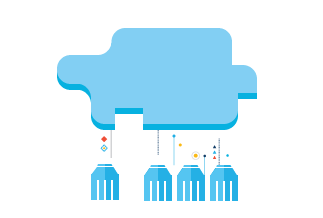
\includegraphics[width=0.4\textwidth]{img/public.png}
    \caption{Nuvem pública~\cite{ibm-what-is-cloud-computing}}
    \label{img:publiccloud}
\end{figure}

Muitos negócios estão usando software como serviço (SaaS) entregue a partir da nuvem 
pública para aplicações que vão de gerenciamento de relacionamento com cliente (CRM) 
a gerenciamento de transação e \emph{analytics} de 
dados~\cite{ibm-what-is-cloud-computing}.

Além de aplicações SaaS, empresas estão usando outros serviços de nuvem pública, 
incluindo infraestrutura como serviço (IaaS) para incluir mais serviços de 
armazenamento ou de computação de imediato e plataforma como serviço (PaaS) para 
ambientes de desenvolvimento e implementação de aplicações baseadas em 
nuvem~\cite{ibm-what-is-cloud-computing}.

Tecnicamente, pode haver pouca ou nenhuma diferença entre a arquitetura de nuvem 
privada e pública. Entretanto, considerações de segurança podem ser substancialmente 
diferentes para os serviços (aplicações, armazenamento e outros recursos) que são 
disponibilizados por um provedor de serviços para um público e quando a comunicação 
é afetada sobre uma rede não confiável~\cite{sequeira2015comptia}. Geralmente, 
provedores de serviços de nuvem pública como a Amazon AWS, Microsoft e Google 
possuem e operam a infraestrutura em seus centros de dados e o acesso geralmente é 
feito por meio da Internet. A AWS e a Microsoft também oferecem serviços conectados 
diretamente chamados "AWS Direct Connect" e "Azure ExpressRoute", respectivamente. 
Tais conexões necessitam que os clientes comprem ou aluguem uma conexão privada a um 
ponto de troca de tráfego oferecido pelo provedor de nuvem 
~\cite{sequeira2015comptia}.

As aplicações de diversos usuários ficam misturadas nos sistemas de armazenamento,
o que pode parecer ineficiente a princípio. Porém, se a implementação de uma nuvem
pública considera questões fundamentais, como desempenho e segurança, a existência
de outras aplicações sendo executadas na mesma nuvem permanece transparente tanto
para os prestadores de serviços como para os usuários~\cite{technet-cloud-computing}.

As características chaves da nuvem pública são, portanto, segurança e controle
sofisticados projetados para os requisitos específicos de uma empresa.

\subsection{Nuvem híbrida}

A nuvem híbrida usa uma base de nuvem privada combinada ao uso estratégico de 
serviços de nuvem pública~\cite{ibm-what-is-cloud-computing}. A realidade é que uma 
nuvem privada não pode existir isolada do restante dos recursos de TI e a nuvem 
pública de uma empresa. A maioria das empresas com nuvens privadas se desenvolverão 
para gerenciar cargas de trabalho entre data centers, nuvens privadas e nuvens 
públicas --- criando, assim, nuvens híbridas~\cite{ibm-what-is-cloud-computing}.

\begin{figure}[ht]
    \centering
    
\includegraphics[width=0.4\textwidth]{img/hybrid.png}
    \caption{Nuvem híbrida~\cite{ibm-what-is-cloud-computing}}
    \label{img:hybridcloud}
\end{figure}

O desenvolvimento para uma estratégia de nuvem híbrida permite com que empresas 
mantenham aplicações críticas para a linha de negócios e dados sigilosos em um 
ambiente de datacenter tradicional ou nuvem privada enquanto também irão tirar 
proveito de recursos da nuvem pública, como SaaS para as aplicações mais recentes e 
IaaS para recurso virtuais econômicos elásticos a serem 
escalados~\cite{ibm-what-is-cloud-computing}.

Nas nuvens híbridas, há uma composição dos modelos de nuvens públicas e privadas. 
Essa característica possui a vantagem de manter os níveis de serviço mesmo que haja 
flutuações rápidas na necessidade dos recursos~\cite{technet-cloud-computing}. A 
conexão entre as nuvens pública e privada pode ser usada até mesmo em tarefas 
periódicas que são mais facilmente implementadas nas nuvens públicas, por 
exemplo~\cite{technet-cloud-computing}. O termo computação em ondas é, em geral, 
utilizado quando se refere às nuvens híbridas~\cite{technet-cloud-computing}.

O fator chave para o sucesso de nuvem híbrida: a capacidade para gerenciar de
forma eficiente e segura a combinação de serviços de nuvem pública e privada
como um único ambiente de computação unificado, tirando proveito integral da
nuvem~\cite{ibm-what-is-cloud-computing}.

\subsection{Nuvem comunitária} Na nuvem comunitária, a infraestrutura de nuvem é 
compartilhada por diversas organizações e suporta uma comunidade específica que 
partilha as preocupações (por exemplo, a missão, os requisitos de segurança, 
política e considerações sobre o cumprimento)~\cite{brown2014seguranca}. Pode ser 
administrado por organizações ou por um terceiro e pode existir localmente ou 
remotamente~\cite{brown2014seguranca}.
